\subsection{Risoluzione delle criticità}

\setLayout{vertical}

\begin{frame}
    \frametitle{Risoluzione delle criticità}
    Abbiamo analizzato approfonditamente l'interfaccia originale, valutandovi linee guida riconosciute e facendola testare a giornalisti. 
    \begin{figure}
        \centering
        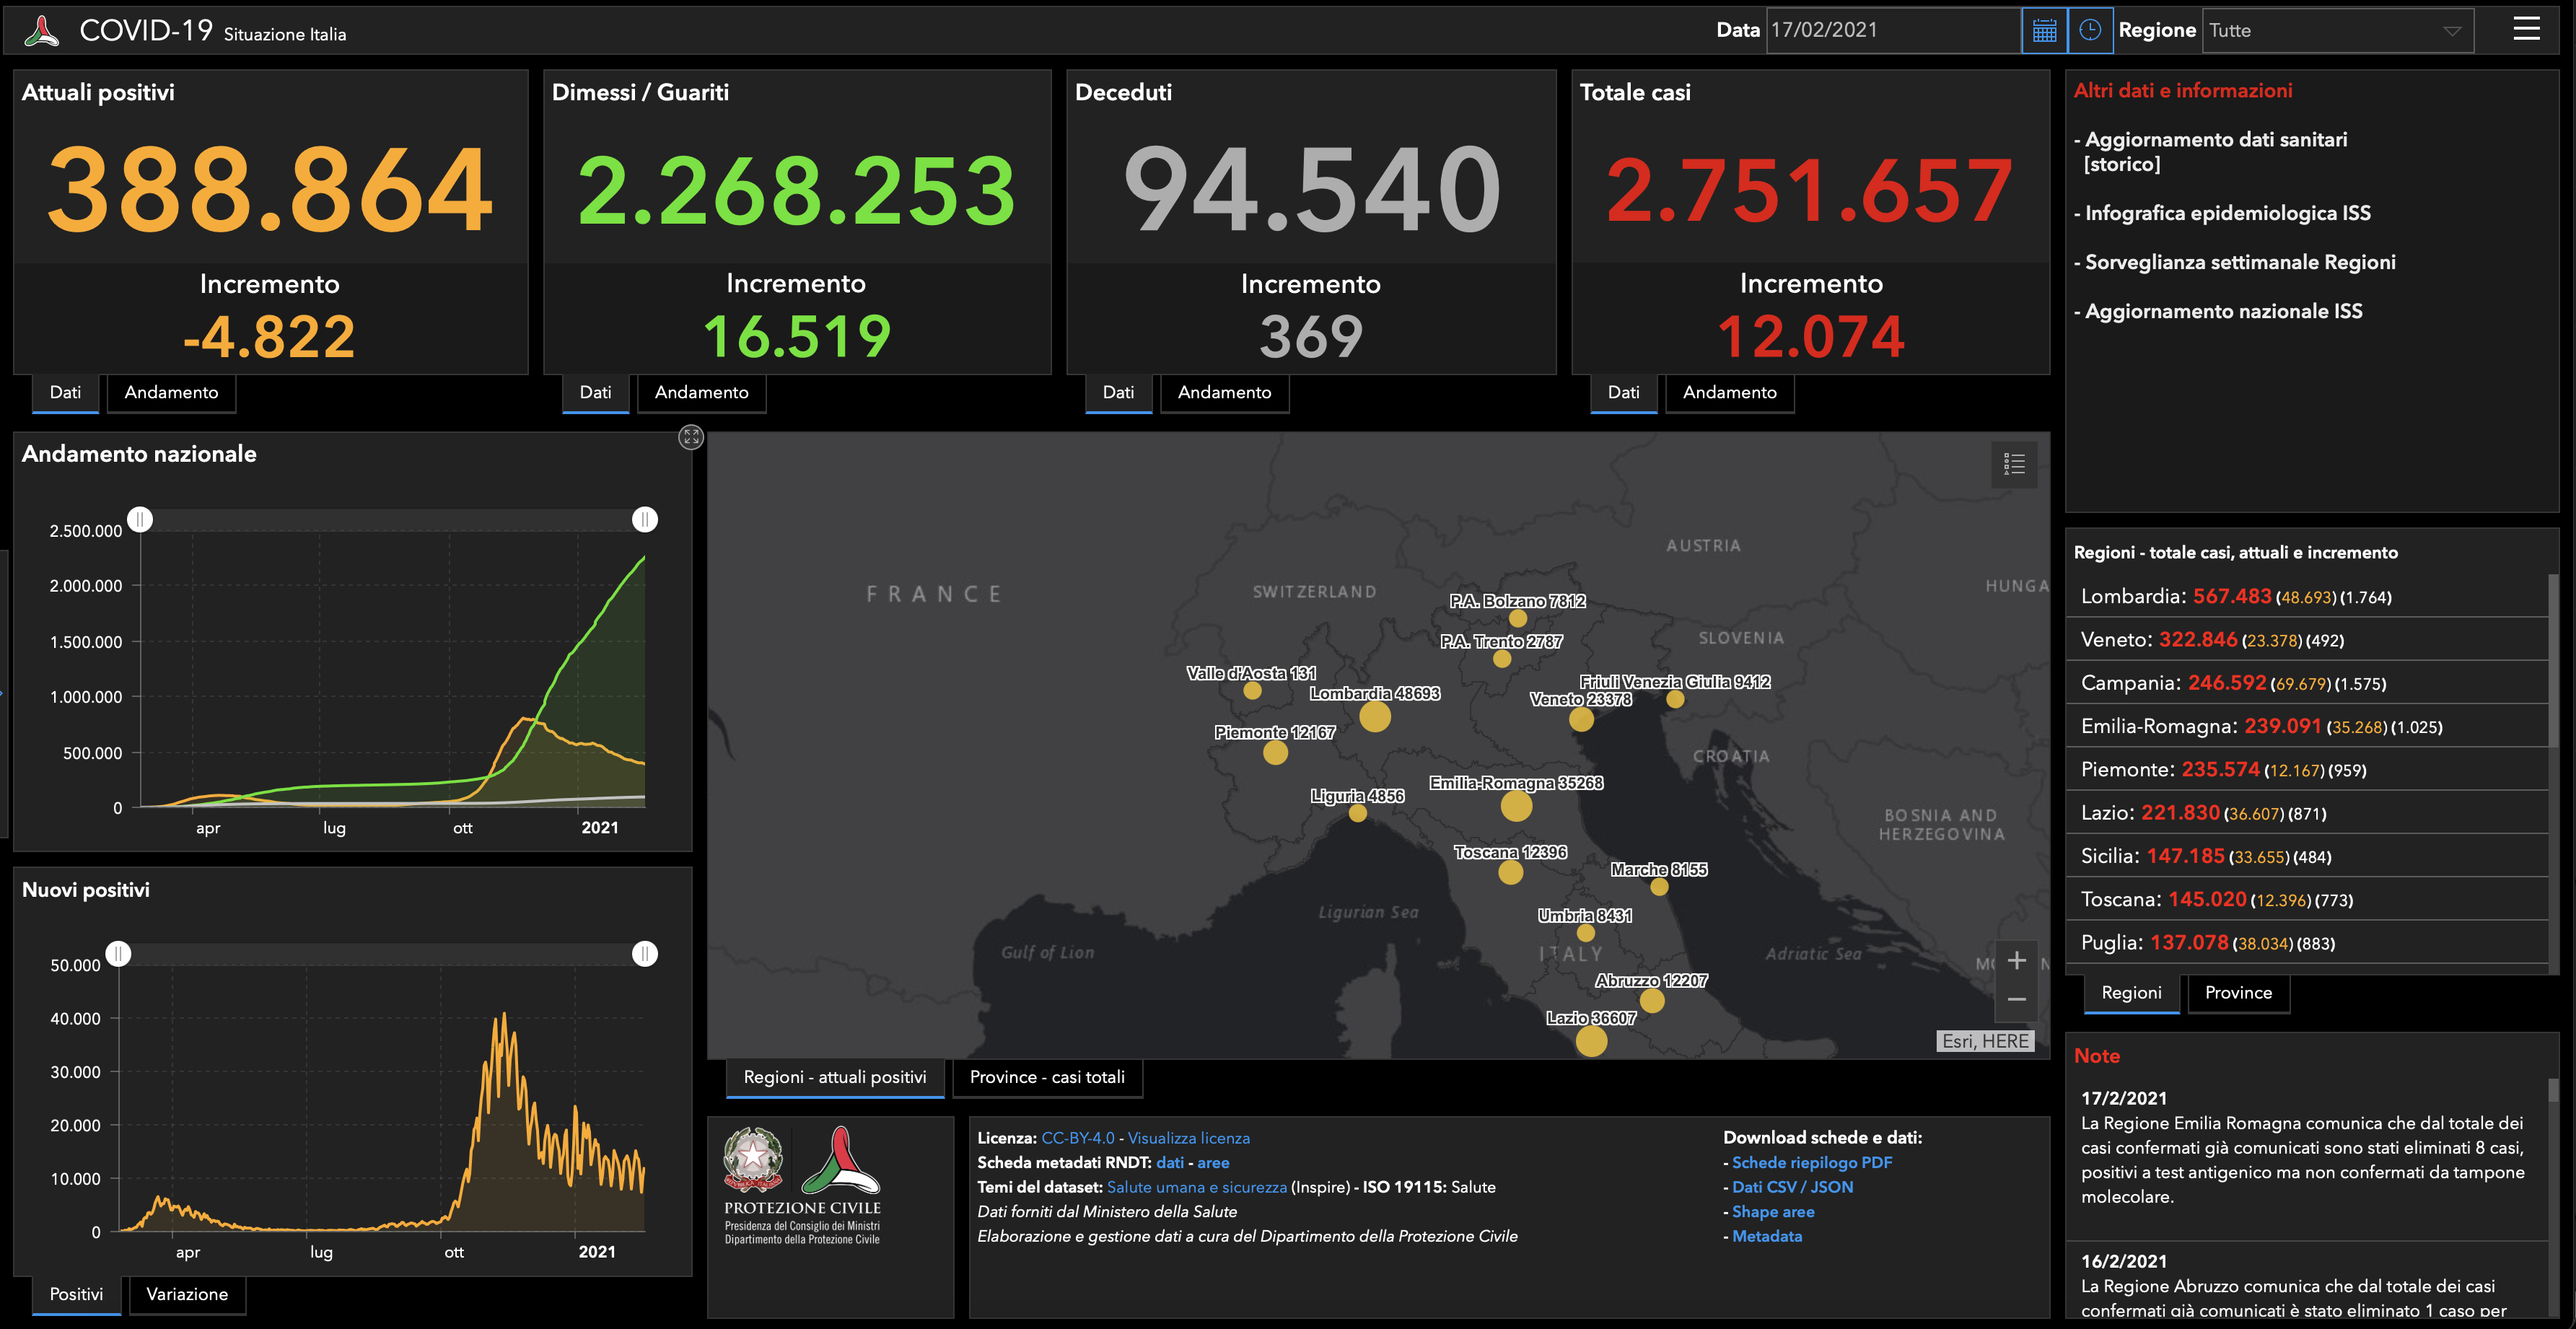
\includegraphics[width=.65\textwidth]{screen-interfaccia/screenshot-dashboard-DPC.png}
        \caption{Screenshot della dashboard del Dipartimento della Protezione Civile catturato il 17 febbraio '21.}
    \end{figure}
\end{frame}

\begin{frame}
    \frametitle{Risoluzione delle criticità}
    Abbiamo individuato le seguenti criticità: 
    \begin{itemize}
        \item<1-> Scarsa leggibilità per scritte piccole e riempimento disomogeneo;
        \item<2-> Distanza tra l'interazione con la mappa e il modello mentale degli utenti;
        \item<3-> Discrepanza tra significante\footnote{Il \textit{significante} è una proprietà di un oggetto che ne rende visibile o ne esplicita l'affordace.} e comportamento effettivo;
        \item<4-> Assenza di meccanismi di prevenzione degli errori nel widget calendario;
        \item<5-> Interazione limitata con la mappa;
        \item<6-> Assenza di componenti grafiche per ridurre carico cognitivo;
        \item<7-> Adozione del colore come unico mezzo distintivo delle componenti;
        \item<8-> Difficoltà dell'interazione coi grafici;
    \end{itemize}    

\end{frame}

\begin{frame}
    \frametitle{Scarsa leggibilità}
    Soluzioni adottate: 
    \begin{itemize}
        \item<1-> abbiamo ingradito la dimensione delle scritte particolarmente piccole e uniformato le dimensioni di tutte le componenti testuali in base alla loro importanza;
        \item<2-> abbiamo evitato la creazione di spazi vuoti, distribuendo tutti gli elementi in maniera omogenea sull'interfaccia;
        \begin{itemize}
            \item<2-> un esempio è la riprogettazione della componente delle note e quelle dei provvedimenti, per le quali abbiamo cambiato il semplice box dell'interfaccia originale in una sidebar on-demand, riuscendo a dare maggiore spazio e leggibilità, senza sacrificare in maniera permanente lo spazio dell'interfaccia;
        \end{itemize}
    \end{itemize}    

\end{frame}

\begin{frame}
    \frametitle{Scarsa leggibilità}
    \begin{figure}
        \centering
        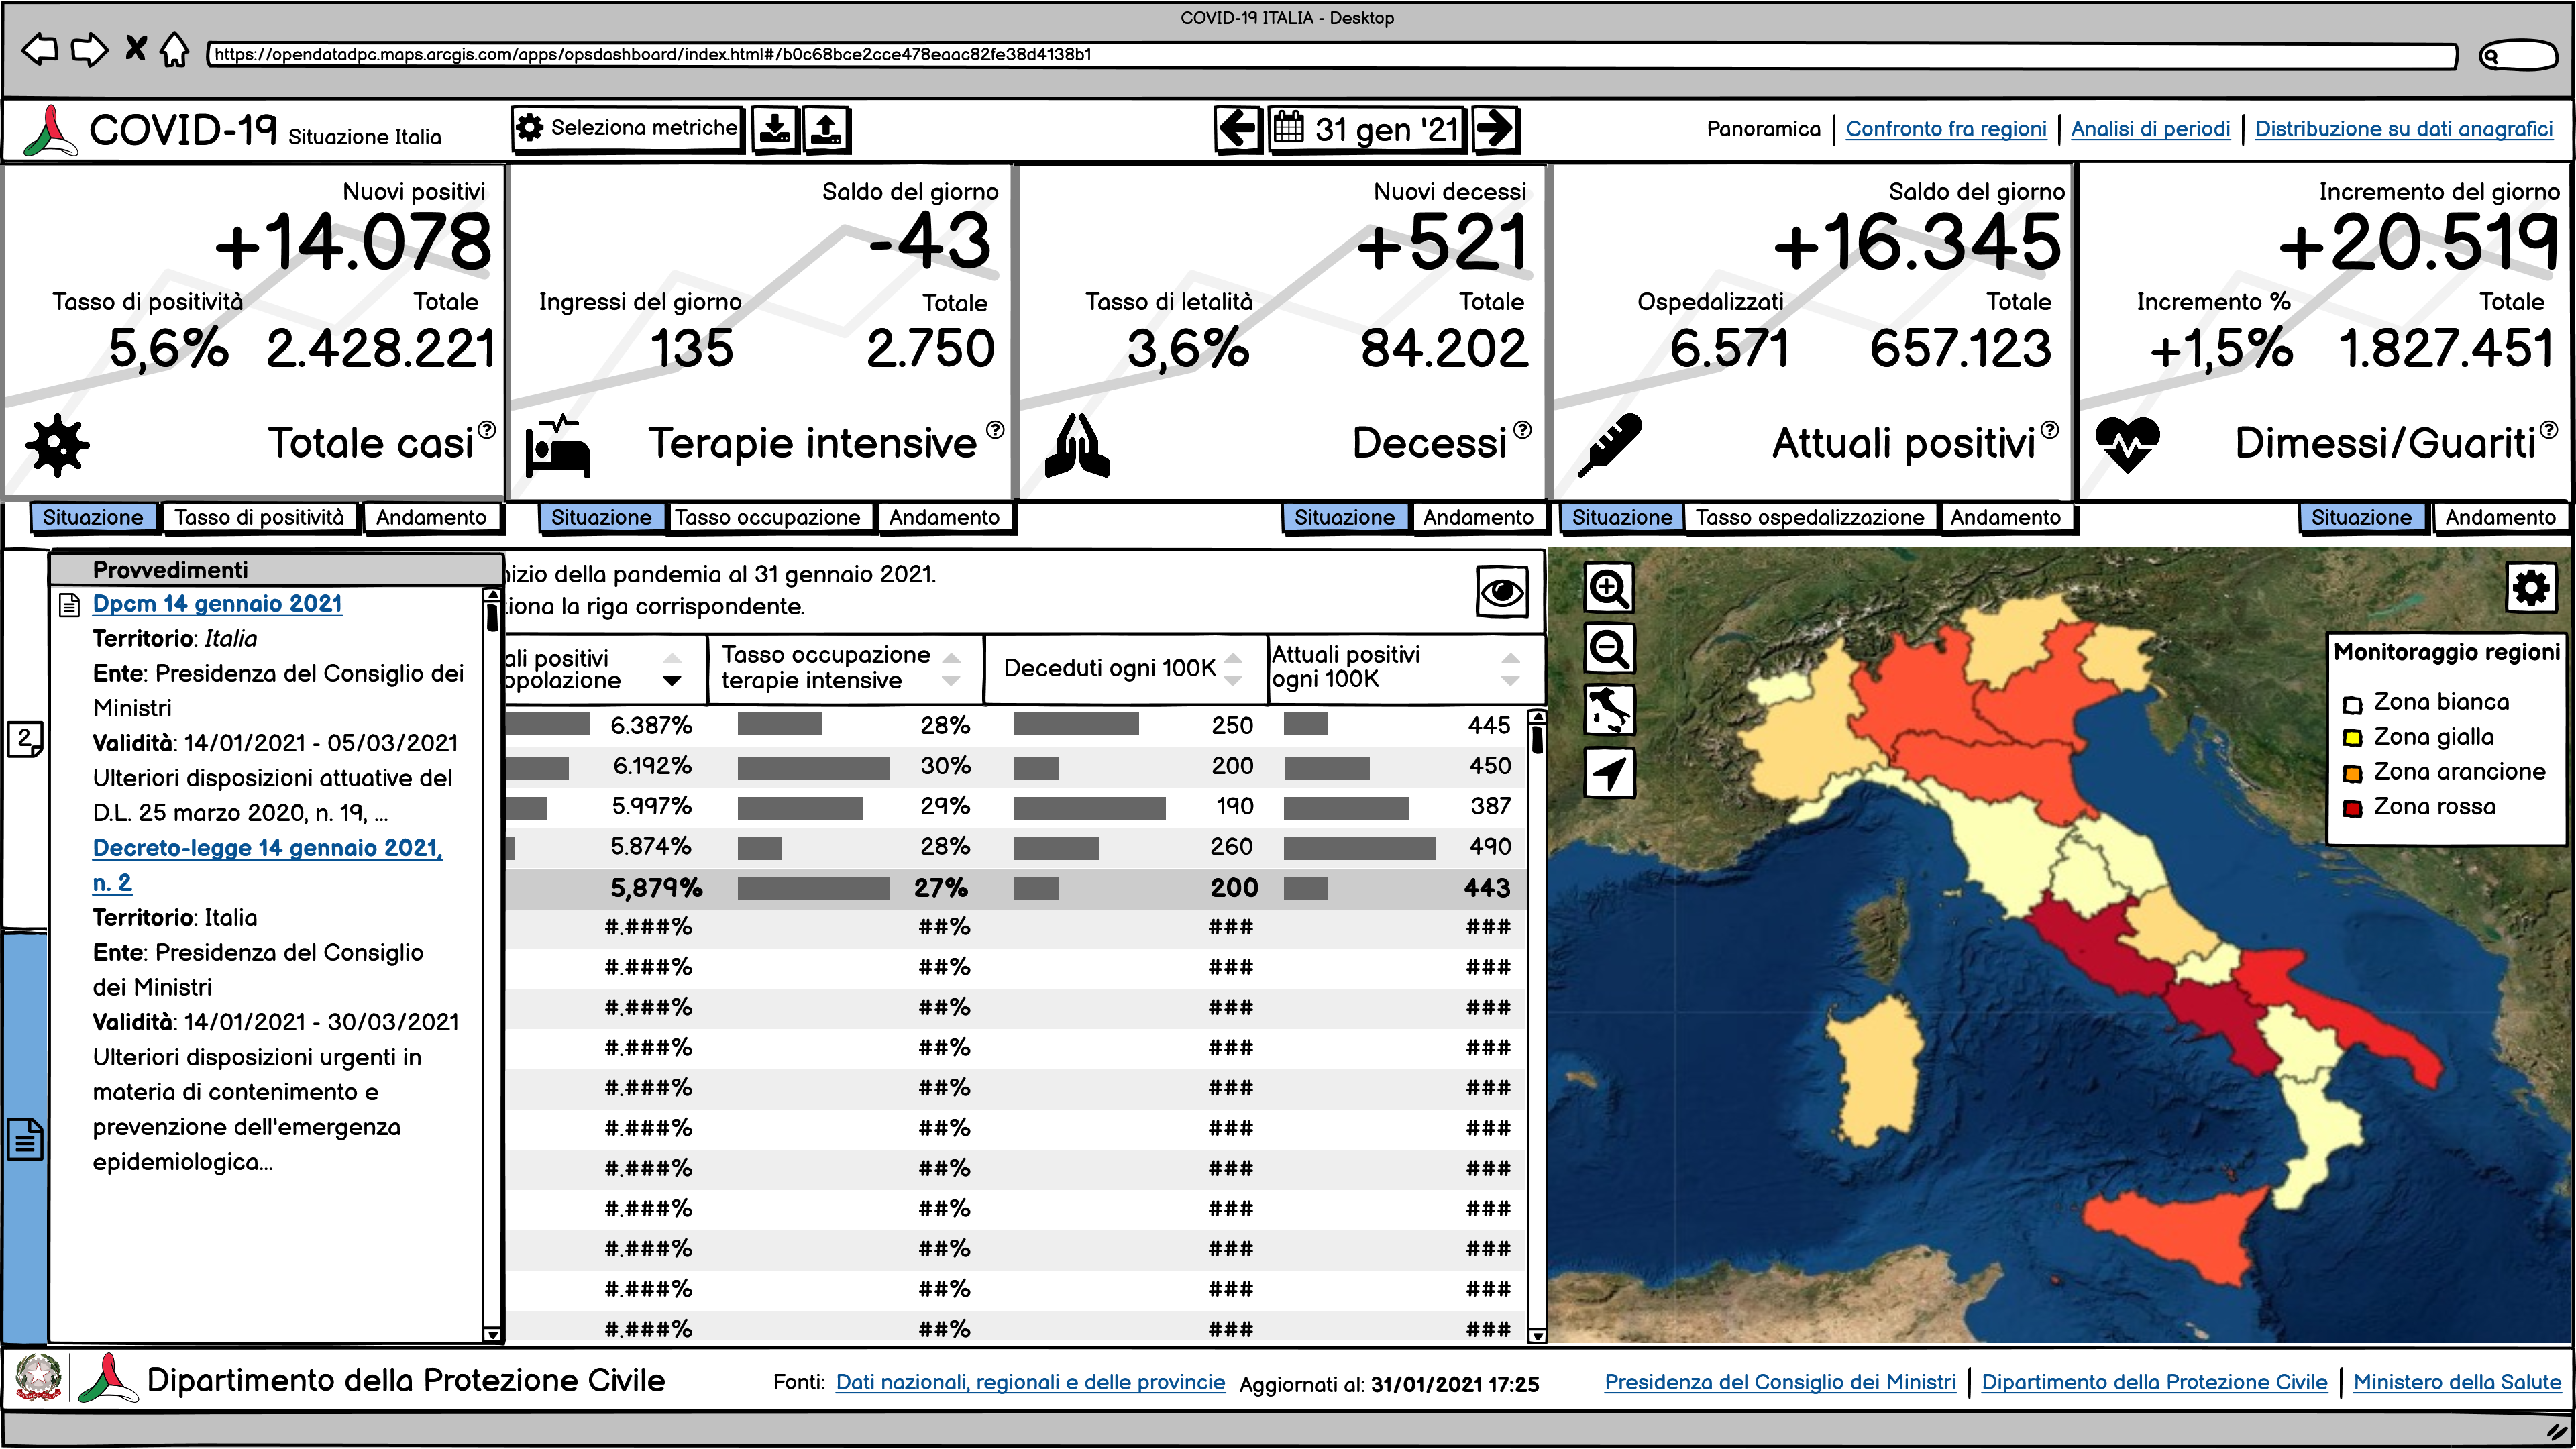
\includegraphics[trim = 0 20 0 55, clip, width=.85\textwidth]{screen-interfaccia/11 - Panoramica.png}
        \caption{Schermata ``Panoramica" della nuova interfaccia con sezione "Provvedimenti" aperta}
    \end{figure}
\end{frame}

\begin{frame}
    \frametitle{Distanza dal modello mentale degli utenti}
    Soluzioni adottate: 
    \begin{itemize}
        \item<1-> 
        \end{itemize}
    \end{itemize}    

\end{frame}